\documentclass{article}

\usepackage{graphicx}
\usepackage{tikz}
\usepackage{tikzsymbols}
\usetikzlibrary{calc,patterns,shapes.geometric}
\pagestyle{empty}
\usepackage[margin=0pt]{geometry}
\geometry{papersize={14in,12in}}

\def\centerarc[#1](#2)(#3:#4:#5){\draw[#1] ($(#2)+({#5*cos(#3)},{#5*sin(#3)})$) arc (#3:#4:#5);}

\begin{document}
	\begin{figure}
		\centering
		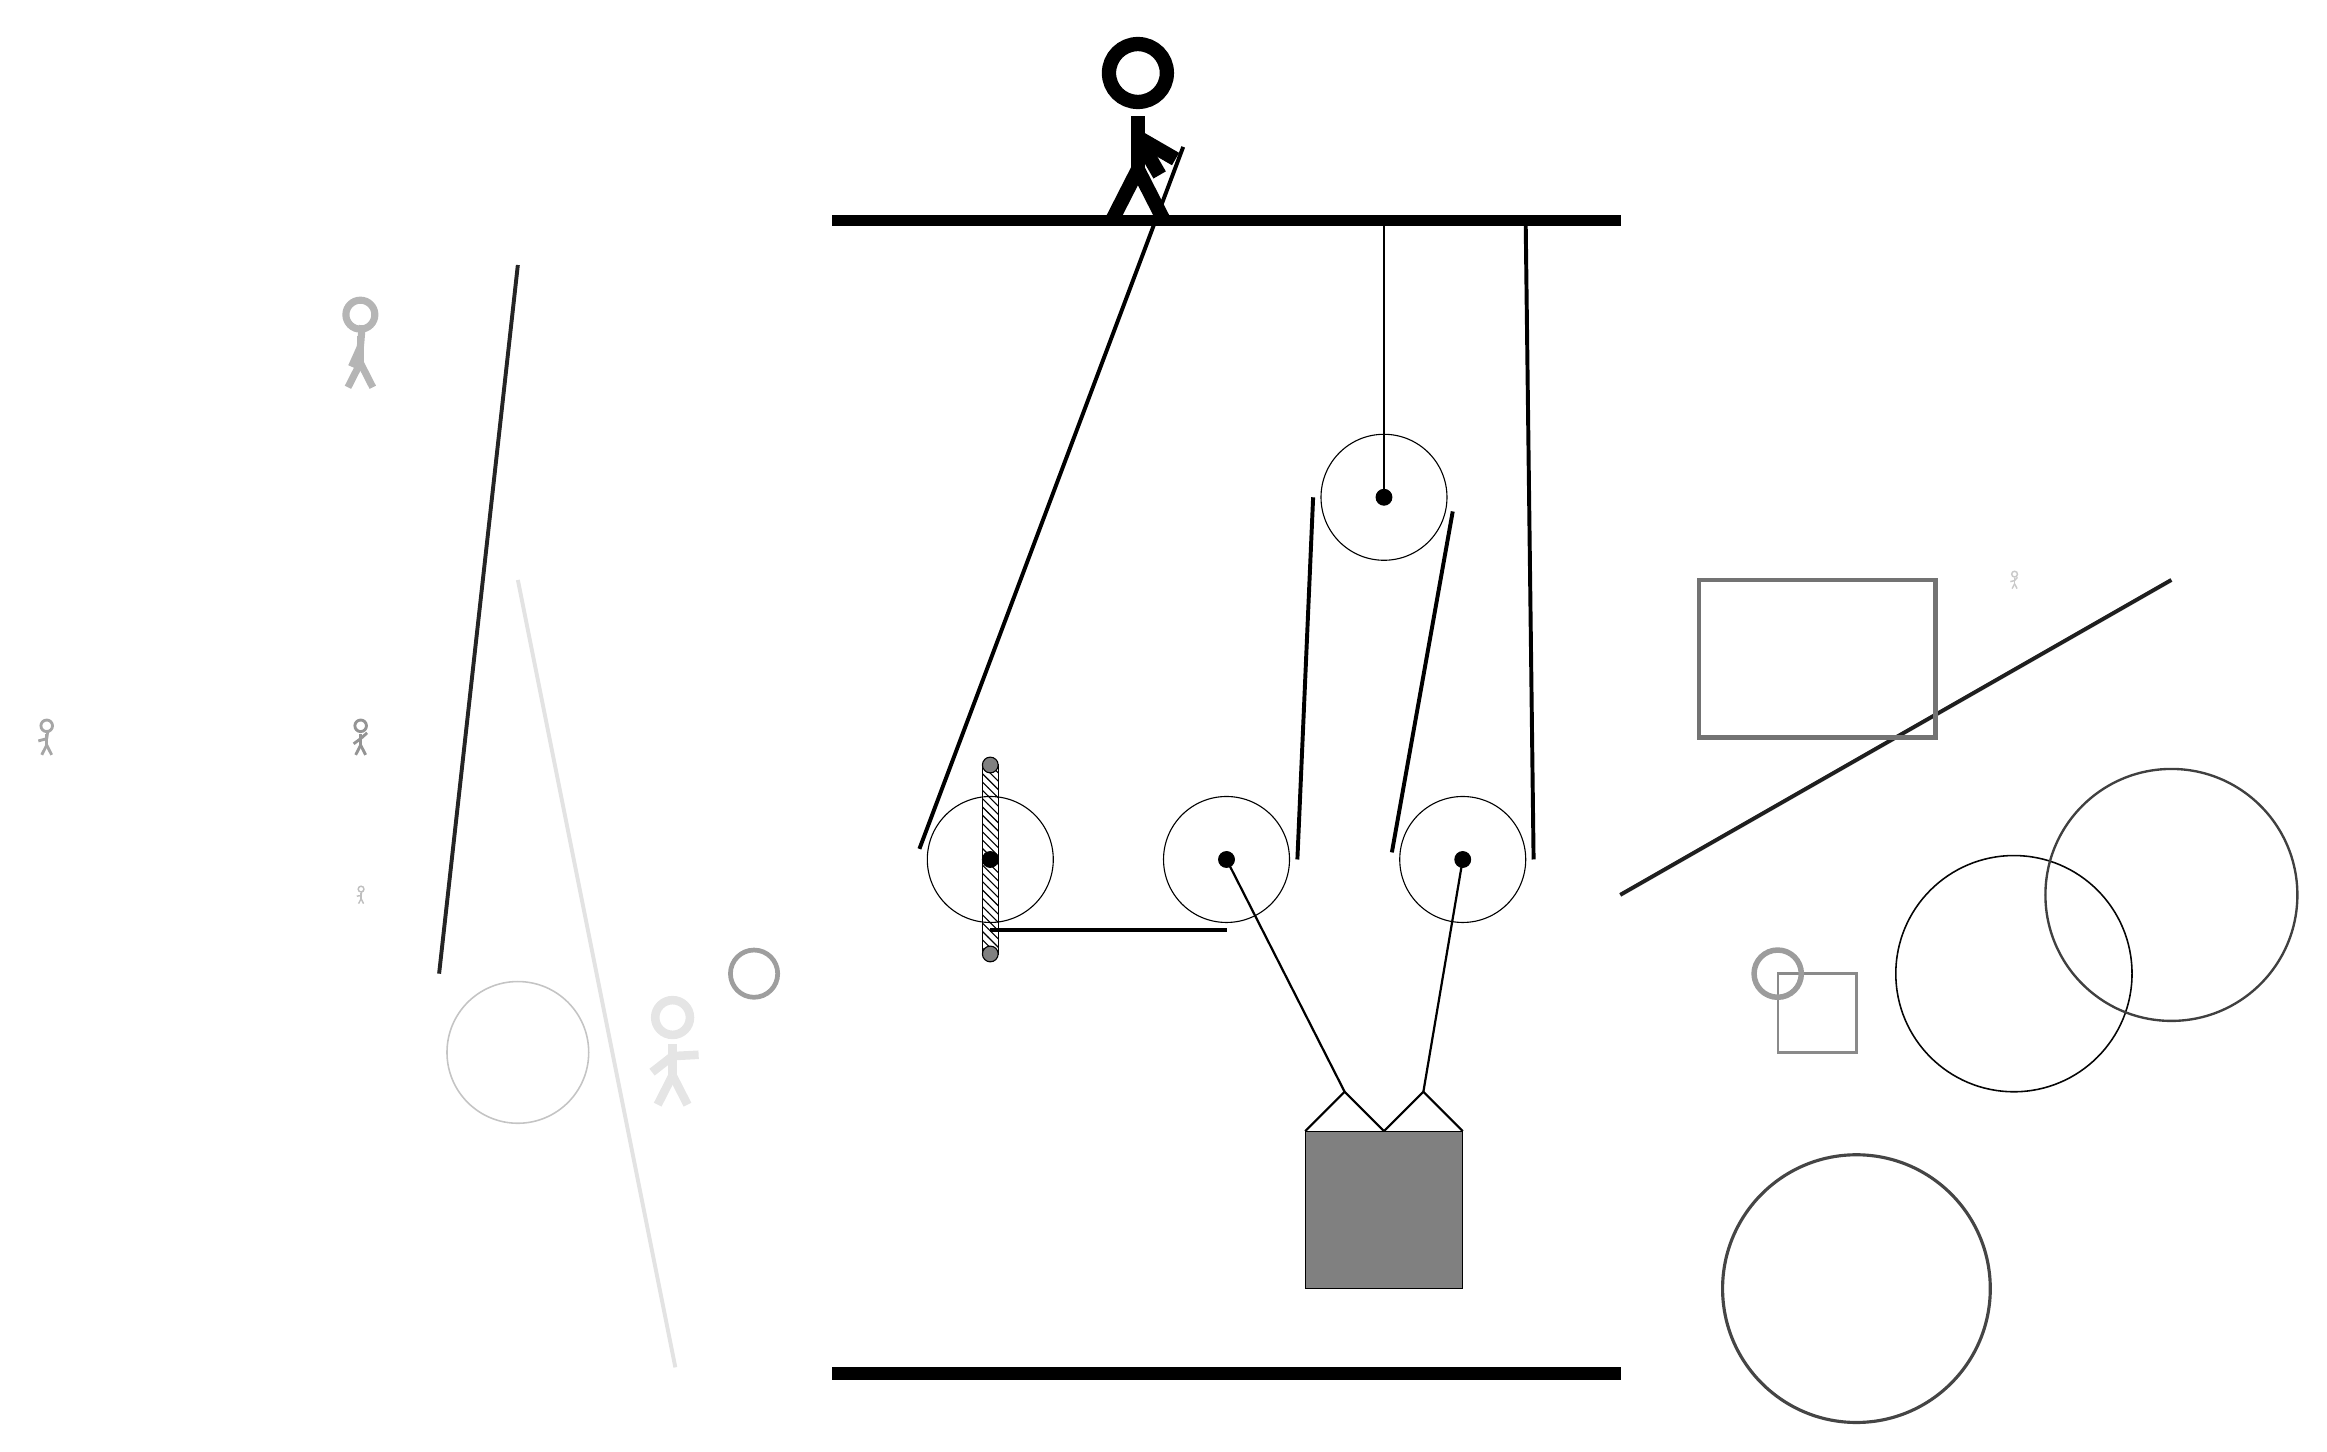
\begin{tikzpicture}
			%%%%% START %%%%%
			
			\draw[fill=black] (-4, 11.5) rectangle (6, 11.625);
			
			\draw (1, 3.45) circle (0.8);
			\draw[fill=black] (1, 3.45) circle (0.1);
			
			\draw (3, 8.05) circle (0.8);
			\draw[fill=black] (3, 8.05) circle (0.1);
			\draw[thick] (3, 8.05) -- (3, 11.5);
			
			\draw (4, 3.45) circle (0.8);
			\draw[fill=black] (4, 3.45) circle (0.1);
			
			\draw[line width=0.5mm, color=black!88](6, 3) -- (13, 7);
			
			\node[line width=0.5mm, color=black!35] at (-14, 5) {\Strichmaxerl[2][15][82]};
			\draw[line width=0.5mm, color=black!11](-6, -3) -- (-8, 7);
			\draw [line width=0.2mm, color=black!23](-8, 1) circle (0.9);
			\draw[line width=0.5mm, color=black!86](-9, 2) -- (-8, 11);
			\node[line width=0.6mm, color=black!42] at (-10, 5) {\Strichmaxerl[2][36][42]};
			\draw [line width=0.2mm, color=black!90](-10, 3) circle (0.0);
			
			\draw [line width=0.2mm, color=black!98](11, 2) circle (1.5);
			\node[line width=0.2mm, color=black!29] at (-10, 10) {\Strichmaxerl[5][66][85]};
			
			\draw[line width=0.6mm, color=black!55] (7, 5) rectangle (10, 7);
			\draw [line width=0.3mm, color=black!75](13, 3) circle (1.6);
			\node[line width=0.5mm, color=black!21] at (11, 7) {\Strichmaxerl[1][14][49]};
			\draw [line width=0.6mm, color=black!38](-5, 2) circle (0.3);
			
			\draw [line width=0.4mm, color=black!73](9, -2) circle (1.7);
			\node[line width=0.3mm, color=black!10] at (-6, 1) {\Strichmaxerl[6][38][3]};
			\draw[line width=0.3mm, color=black!46] (8, 2) rectangle (9, 1);
			\node[line width=0.3mm, color=black!25] at (-10, 3) {\Strichmaxerl[1][8][81]};
			
			\draw [line width=0.7mm, color=black!39](8, 2) circle (0.3);
			
			\draw[thick] (4, 3.45) -- (3.5, 0.5);
			\draw[thick] (1, 3.45) -- (2.5, 0.5);
			\draw[thick]  (2, 0) -- (2.5, 0.5) -- (3, 0);
			\draw[thick]  (3, 0) -- (3.5, 0.5) -- (4, 0);
			\draw[fill=black!50] (2, 0) rectangle (4, -2);
			
			\draw (-2, 3.45) circle (0.8);
			\draw[fill=black] (-2, 3.45) circle (0.1);
			\draw[pattern=north west lines, pattern color=black] (-2.1, 4.65) rectangle (-1.9, 2.25);
			\draw[fill=black!50] (-2, 4.65) circle (0.1);
			\draw[fill=black!50] (-2, 2.25) circle (0.1);
			
			\draw[line width=0.5mm] (0.45, 12.5) -- (-2.9, 3.585);
			\centerarc[line width=0.5mm](-2, 3.45)(160:270:0.9);
			\draw[line width=0.5mm](-2, 2.55) -- (1, 2.55);
			\centerarc[line width=0.5mm](1, 3.45)(270:360:0.9);
			\draw[line width=0.5mm] (1.9, 3.45) -- (2.1, 8.05);
			\centerarc[line width=0.5mm](3, 8.05)(-20:180:0.9);
			\draw[line width=0.5mm](3.873, 7.87) -- (3.1, 3.54);
			\centerarc[line width=0.5mm](4, 3.45)(160:360:0.9);
			\draw[line width=0.5mm](4.9, 3.45) -- (4.8, 11.5);
			
			\node at (-0.07, 12.7) {\Strichmaxerl[10][120][-30]};
			
			\draw[fill=black] (-4, -3) rectangle (6, -3.15);
			
			%%%%% END %%%%%
		\end{tikzpicture}
	\end{figure}	
\end{document}